\documentclass[../seminar.tex]{subfiles}


\begin{comment}


\documentclass{ferseminar}
\usepackage{subfiles}
\usepackage[bottom]{footmisc}
\usepackage{graphicx}
\usepackage{caption}
\usepackage{subcaption}
\graphicspath{{../Slike/}}
\end{comment}

\begin{document}

Jedna od prednosti korištenja stereo sustava kamera je mogućnost samo-kalibracije (engl. \textit{self-calibration, auto-calibration}).
Samo-kalibracija je proces izračuna unutrašnjih parametara kamere pomoću slika neke nestrukturirane scene. Za razliku od 'klasične' kalibracije 
ona ne zahtijeva posebne kalibracijske uzorke. Glavna pretpostavka samo-kalibracije je da se slike projiciraju iz euklidskog prostora kroz \textit{pinhole} model kamere s nelinearnim izobličenjem. 
Linearni \textit{pinhole} parametri su žarišna duljina, omjer slike (engl. \textit{aspect ratio}), iskrivljenost (engl. \textit{skew}) i glavna 2D točka (engl. \textit{2D principal point}).
Koristeći niz kalibriranih ili nekalibriranih slika scena se može rekonstruirati sve do šest stupnjeva euklidske transformacije i izotropnog skaliranja.\cite{Hartley}


U \cite{Abraham} se koristila samo-kalibracija pomoću kalibracijskog uzorka (Slika \ref{fig:calibration_board}) s tri ravnine (što nije nužno, ali pospješuje rezultate).
Na ravninama su se nalazile iscrtane točke s približno poznatim međusobnim udaljenostima. Uzorak se snimao nekoliko puta sa stereo sustavom kamera s ribljim okom nakon čega 
su se pomoću programskog procesa izračunali parametri modela rektifikacije i estimirale koordinate 3D točaka. Točke su se grupirale u grupe od četiri točaka čime se omogućilo
automatsko dekodiranje. Za svaku sliku su se aproksimirale vrijednosti vanjske i unutarnje orijentacije pomoću direktne linearne transformacije (DLT, engl. \textit{Direct Linear Transformation})
koja u sebi ima ugrađen ekvidistantan projekcijski model. U tom dijelu postupka kalibracije su korištene i otprije poznate približno poznate pozicije stvarnih 3D točaka.


\begin{figure*}[ht!]
  \centering
    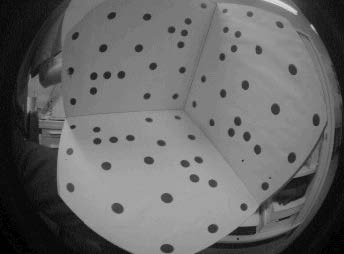
\includegraphics[width=.5\textwidth]{img_012_calibration_board.png}
   \caption{Kalibracijski uzorak s tri ravnine (izvor: \cite{Abraham})}
  \label{fig:calibration_board}
\end{figure*}




Nakon prikupljanja izračunatih vrijednosti $\boldsymbol{x'}_{L_{ij}}$ i $\boldsymbol{x'}_{R_{ij}}$ iz svih slika $j$ za točke $i$, intrinsičnih parametara $\hat{\boldsymbol{p}}_{CL}$ i $\hat{\boldsymbol{p}}_{CR}$ 
lijeve i desne kamere, omjer stereo parametara $(\hat{\boldsymbol{R}},\hat{\boldsymbol{t}})_{CL,CR}$, extrinzični parametri $(\hat{\boldsymbol{R}},\hat{\boldsymbol{t}})_{W,CL_j}$ 
i koordinate točaka $\hat{\boldsymbol{X}}_{W_i}$ se estimiraju simultano pomoću nelinearnog iterativnog samo-kalibrirajućeg postupka. Preinake minimiziraju reprojekcijsku pogrešku $\Omega$ između 
projekcijskog modela i stvarnih mjerenja:

\begin{equation}
\label{eq:reprojection_error_minimization}
\Omega = \sum\limits_{i}\sum\limits_{j}[\boldsymbol{x}'_{L_{ij}} - \boldsymbol{f}(\hat{\boldsymbol{p}}_{CL},(\hat{\boldsymbol{R}},\hat{\boldsymbol{t}})_{W,CL_j},\hat{\boldsymbol{X}}_{W_i})]^2 + [\boldsymbol{x}'_{R_{ij}} - \boldsymbol{f}(\hat{\boldsymbol{p}}_{CR},(\hat{\boldsymbol{R}},\hat{\boldsymbol{t}})_{W,CL_j},(\hat{\boldsymbol{R}},\hat{\boldsymbol{t}})_{CL,CR},\hat{\boldsymbol{X}}_{W_i})]^2
\end{equation}

Kako bi se dobio što bolji rezultat potrebno je odabrati projekcijski model za riblje oko. U \cite{Abraham} su odabrali onaj koji najbolje odgovara 
podacima pomoću estimirane srednje reprojekcijske pogreške $\hat{\sigma}_{x'} = \sqrt{\Omega/r}$  ($r$ je redundancija) sustava.

Ako zanemarimo projekcijski model ribljeg oka kalibracijski postupak je jednak standardnom samo-kalibracijskom postupku. 

Nakon kalibracije slijedi rektifikacija slika i izračun tablica s predizračunatim vrijednostima (engl. \textit{look-up-tables}). 


\subsection{Primjer implementacije rektifikacije i stereo kalibracije}

Primjer iz \cite{Abraham} demonstrira kalibraciju, rektifikaciju i 3D-rekonstrukciju pomoću uparenih kamera s ribljim okom. Slika \ref{fig:calib_rect_examples} prikazuje originalan par slika i njihove različite epipolarne rektifikacije.
Na slici se može uočiti mnogo manje izobličenje neperspektivnih projekcija naspram perspektivne projekcije. Posljedica toga je lakše stereo uparivanje točaka slika. Razlike između izobličenja epipolarne ekvidistantne i stereografske projekcije su male. U \cite{Abraham} ti modeli imaju gotovo jednake performanse i rezultate u kontekstu stereo uparivanja.

Kalibracija se obavila na prethodno opisan način. Koristila se radijalna projekcijska funkcija $r' = sin(\theta / 2)$. 

\begin{table}[h]
\centering
\begin{tabular}{ ccc  }

 \hline
 \multicolumn{3}{c}{Intrinsični parametri} \\
 \hline
 & lijeva kamera & desna kamera\\
 \hline
 $c_x$   & 308.8 (0.5) & 311.0 (0.6)\\
 $c_y$ & 308.3 (0.5) & 310.7 (0.5)\\
 $x'_H$ & 245.78 (0.03) & 251.67 (0.02)\\
 $y'_H$ & 129.2 (0.03) & 125.56 (0.02)\\

 \hline
\end{tabular}
\label{table:table_intrinsic}
\end{table}

\begin{table}[h]
\centering
\begin{tabular}{ cccc  }

 \hline
 \multicolumn{4}{c}{Relativna orijentacija} \\
 \hline
 $t_x [mm]$   & 78.64 (0.05) & $r_x$ & 0.17° (0.01°)\\
 $t_y [mm]$ & 0.42 (0.03) & $r_y$ & 1.56° (0.02°)\\
 $t_z [mm]$ & 0.62 (0.06) & $r_z$ & 0.15° (0.01°)\\
 
\end{tabular}
\caption{Tablica vrijednosti intrinsičnih parametara i relativne orijentacije}
\label{table:table_relative}
\end{table}

Tablica (\ref{table:table_relative}) prikazuje estimirane parametre kalibracije s njihovim standardnim devijacijama. Estimirana usrednjena reprojekcijska pogreška je iznosila $\hat{\sigma}_{x'} = 0.13$.



\begin{figure*}[ht!]
  \centering
    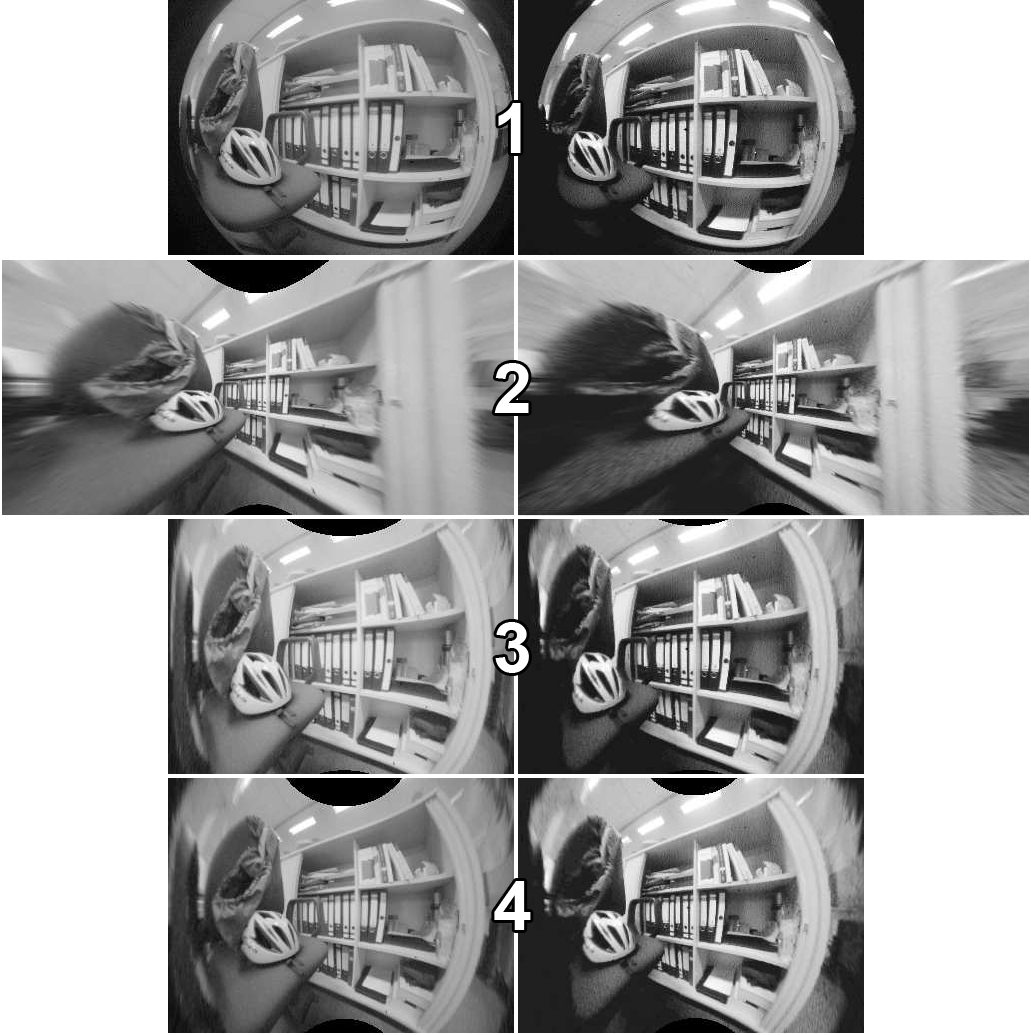
\includegraphics[width=.9\textwidth]{calib_rect_examples.png}
   \caption{Primjeri rektifikacija originalnog para slika (1): perspektivna (2), ekvidistantna (3) i stereografska (4) (izvor: \cite{Abraham})}
  \label{fig:calib_rect_examples}
\end{figure*}

Nakon kalibracije i rektifikacija napravljena je 3D-rekonstrukcija pomoću para slika. Korišten je model epipolarne stereografske projekcije $r' = c * tan(\frac{\theta}{2})$. Rezultat rekonstrukcije se može vidjeti na Slici \ref{fig:calib_rect_examples}. Ona prikazuje presjek oblaka 3D-točaka (engl \textit{3D-point-cloud}) i presjek na korištenom paru slika. Na dobivenoj slici točaka se mogu uočiti kaciga i rub polica s knjigama. Vidno polje je veličine ~150° no ograničeno je optičkim uređajem pomoću kojih su napravljene slike, ne i rektifikacijskim modelom.

\begin{figure*}[ht!]
  \centering
    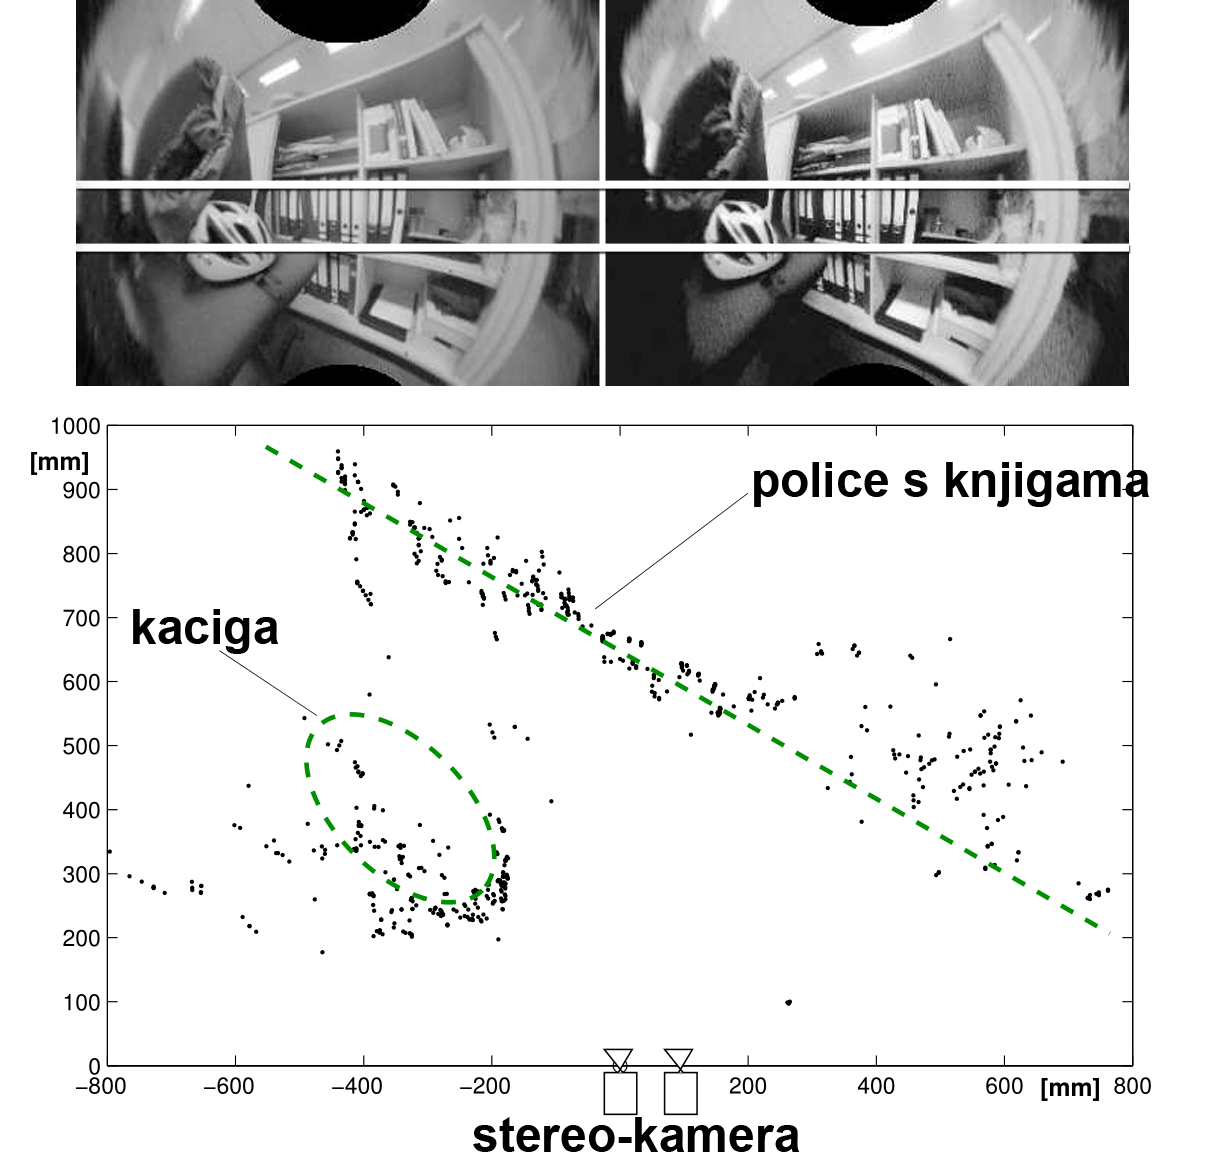
\includegraphics[width=.9\textwidth]{example_helmet_bookcase.png}
   \caption{Horizontalni presjek slika i oblaka 3D-točaka (izvor: \cite{Abraham})}
  \label{fig:calib_rect_examples}
\end{figure*}

\end{document}
